\documentclass[uplatex,a4j,11pt,dvipdfmx]{jsarticle}
\bibliographystyle{jplain}

\usepackage{url}

\usepackage{graphicx}
\usepackage{gnuplot-lua-tikz}
\usepackage{pgfplots}
\usepackage{tikz}
\usepackage{amsmath,amsfonts,amssymb}
\usepackage{bm}
\usepackage{siunitx}

\makeatletter
\def\fgcaption{\def\@captype{figure}\caption}
\makeatother
\newcommand{\setsections}[3]{
\setcounter{section}{#1}
\setcounter{subsection}{#2}
\setcounter{subsubsection}{#3}
}
\newcommand{\mfig}[3][width=15cm]{
\begin{center}
\includegraphics[#1]{#2}
\fgcaption{#3 \label{fig:#2}}
\end{center}
}

\begin{document}
%\section{実験原理}
%\subsubsection*{(3-1)}
実験により$660\ \si{\kilo\metre}$の温度,圧力においてクラペイロン勾配が負の相転移があることがわかっている.
この相転移では温度が高いほど高密度相への相転移に必要な圧力が低い.
すると平均温度のマントルが高密度相に相転移できる深さに至っても低温のマントルが低密度相のままということになる.
また平均より温度が高いマントルは上昇して圧力が下がっても低密度相に相転移しにくくなる.
以上から低温のマントルは周囲に比べて軽く,高温のマントルが周囲に比べて重くなるため,対流が阻害されるのである.
\subsubsection*{(3-2)}
プレートの沈み込み境界では地震活動が起こりやすいが,多くの沈み込み境界において震源深さは$670\ \si{\kilo\metre}$程度まででそれ以上深い地震は観測されていない.
これは$670\ \si{\kilo\metre}$付近でスラブの沈み込みが止まっていることを示唆する.
\subsubsection*{(3-3)}
2層対流では上層と下層において対流が阻害され,その間での熱伝達は伝導が支配的ということになる.
これにより全層対流の時の温度勾配は図(b)のように球殻内部での温度がほぼ一様であったのに比べて,
2層対流では間に遷移層,すなわち温度勾配が急な箇所が発生すると考えられる.
\mfig[width=6cm]{fig/3-3.png}{全層対流と2層対流の場合の温度勾配\cite{kawakatu}}
\subsubsection*{(4-1)}
$n=0$のLegendre陪関数は定数であり0次成分の磁気ポテンシャルに由来する磁場は一方向を向いた磁場になる.
これは磁気単極子成分であり,現実には存在しないことから$n=0$の成分は含まれない.
\subsubsection*{(4-2)}
磁気ポテンシャルは以下のように表される.
\begin{align}
  V=a\left(\left(\frac{a}{r}\right)^2g_1^0\cos\theta+\left(\frac{a}{r}\right)^3g_2^0\frac{1}{2}(3\cos^2\theta-1)\right)
\end{align}
したがって磁束密度の各成分は以下のように表される.
\begin{align}
  B_r=-\frac{\partial V}{\partial r}=2\frac{a^3}{r^3}g_1^0\cos\theta+\frac{3}{2}\frac{a^4}{r^4}g_2^0(3\cos^2\theta-1)
\end{align}
\begin{align}
  B_\theta=-\frac{1}{r}\frac{\partial V}{\partial \theta}=\frac{a^3}{r^3}g_1^0\sin\theta-3\frac{a^4}{r^4}g_2^0\cos\theta\sin\theta
\end{align}
\begin{align}
  B_\varphi=0
\end{align}
ここで地表面においては$a/r=1$である.以上から北極点($\theta=0,\varphi=0$),南極点($\theta=0\pi,\varphi=0$)における磁場$\bm B_N$と$\bm B_S$は極座標において以下のようになる.
\begin{align}
  {\bm B_N}=\left(\begin{array}{c}
    2g_1^0+3g_2^0\\0\\0
  \end{array}\right)=\left(\begin{array}{c}
    -603.8\\0\\0
  \end{array}\right)\ \si{\nano\tesla}
\end{align}
\begin{align}
  {\bm B_S}=\left(\begin{array}{c}
    -2g_1^0+3g_2^0\\0\\0
  \end{array}\right)=\left(\begin{array}{c}
    156.2\\0\\0
  \end{array}\right)\ \si{\nano\tesla}
\end{align}
\subsubsection*{(4-3)}
(4-2)の結果から地軸上において水星の地磁気は動径方向成分のみを持ち,角度成分を持たないことがわかる.
このことから磁気モーメントは地軸に平行になる.磁気双極子が十分狭い範囲に集中しているならば,地表面での磁気双極子による磁束密度は以下のように表される.
\begin{align}
  B=\frac{{\bm m}\cdot{\bm r}}{4\pi r^3}
\end{align}
したがって
\begin{align}
  B\propto\frac{\cos\theta}{r^2}
\end{align}
である.ここで図のように座標を設定すれば
\begin{align}
  \begin{split}
    603.8:156.2&=\frac{1}{x^2}:\frac{1}{(a-x)^2}\\
    x&=822.6\ \si{\kilo\metre}
  \end{split}
\end{align}
したがって磁気双極子は北極点から地軸上で$822.6\ \si{\kilo\metre}$離れた位置に存在することになる.
よって,水星の地磁気は北極側に大きく偏っていることがわかる.
\mfig[width=8cm]{fig/4-3.png}{地軸上の座標の設定}
%\subsubsection*{問題(3)}
1つのフェルミ粒子が持つ磁気モーメントを$\mu_B$とする.フェルミ温度$T_F=\epsilon_F/k_B$
を使ってこの系の低温でのゼロ磁場スピン磁化率を求めよ.\\
\hrulefill
\subsubsection*{解答}
問題4.6 (4)の結果を用いると
\begin{align}
  \begin{split}
    \chi(T)&=2\mu_B^2D(\epsilon_F)\left(1+\frac{\pi^2}{6}(k_BT)^2\frac{{\rm d}^2\ln D(\epsilon)}{{\rm d}\epsilon^2}+\cdots\right)\\
    &=\frac{\mu_B^2\epsilon_F^2}{\hbar^3\omega^3}\left(1+\frac{\pi^2}{6}(k_BT)^2\left(\frac{1/\hbar^3\omega^3}{\epsilon_F^2/2\hbar^3\omega^3}-\frac{(\epsilon_F/\hbar^3\omega^3)}{(\epsilon_F^2/2\hbar^3\omega^3)^2}\right)+\cdots\right)\\
    &=\frac{\mu_B^2\epsilon_F^2}{\hbar^3\omega^3}\left(1+\frac{\pi^2}{6}(k_BT)^2\left(-\frac{2}{\epsilon_F^2}\right)+\cdots\right)\\
    &=\frac{\mu_B^2\epsilon_F^2}{\hbar^3\omega^3}\left(1+\frac{\pi^2}{3}\left(\frac{T}{T_F}\right)^2+O\left(\left(\frac{T}{T_F}\right)^4\right)\right)
  \end{split}
\end{align}
%\section{太陽電波観測}
\subsection{原理}
\subsubsection{回路方程式}
図\ref{fig:04/1-b.png}に非反転増幅器の回路図を示す.
仮想短絡を考えるとオペアンプの-端子の電圧$v_{-}]$は入力電圧$v_i$と等しいと考えられる.
さらに$v_-$は$v_o$を$R_1$と$R_2$で分圧した電圧になるので
\begin{align}
  \begin{split}
    \label{equ:amp_circuit_eq}
    v_i=v_-&=\frac{R_1}{R_1+R_2}v_o\\
    v_o&=\left(1+\frac{R_2}{R_1}\right)v_i
  \end{split}
\end{align}
となる.以上から非反転増幅器は入力信号に対して位相がそのままで,電圧が$1+R_2/R_1$倍の信号が出力されることがわかる.
\mfig[width=10cm]{04/1-b.png}{非反転増幅器}
\subsubsection{伝達関数}
(\ref{equ:amp_circuit_eq})から伝達関数を求めると以下のようになる.
\begin{align}
  \begin{split}
    V_o&=\left(1+\frac{R_2}{R_1}\right)V_i\\
    G(s)=\frac{V_o}{V_i}&=1+\frac{R_2}{R_1}
  \end{split}
\end{align}
これに図\ref{fig:04/1-b.png}で示した値を代入してBode線図を描くと図\ref{fig:graph/1-B/theo-bode.tex}のようになる.
\gnu{Bode線図の理論値}{graph/1-B/theo-bode.tex}

\subsection{方法}
\subsubsection{測定1-B-01}
図\ref{fig:04/1-b.png}の回路をQucs Spice上で作成しDC bias Simulationを行った.
まず$R_1=1.034\ \si{\kilo\ohm}$, $R_2=5.025\ \si{\kilo\ohm}$
として電圧利得6倍の非反転増幅器を構成した.この非反転増幅器上で入力電圧$V_i$を$-3\ \si{\volt}$から$3\ \si{\volt}$まで$0.5\ \si{\volt}$
刻みで変化させながら出力電圧$V_o$を記録した.
\subsubsection{測定1-B-02}
上記の回路で$R_2$を$608.4\ \si{\ohm}$に変更し,電圧利得1.6倍の非反転増幅器を構成した.
この回路においてTransient Simulationを行った.
この回路に$V_{p-p}=1\ \si{\volt}$,周波数が$10$, $100$, $1\si{\kilo}$, $10\si{\kilo}$, $100\ \si{\kilo\hertz}$の正弦波を入力し利得及び位相差を記録, Bode線図を作成した.
また周波数が$1\ \si{\kilo\hertz}$の時の波形を記録した.
\subsection{測定3:FPIによるレーザー光の分光}
表\ref{tab:kyosinki_Tt}に共振器長$D$と$T$, $t$の関係を示す.
また図\ref{fig:graph/day3/day3_02.tex}に$D$と$t/T$の関係を示す.
\begin{table}[h]
\caption{共振器長と$T$, $t$の関係}
\label{tab:kyosinki_Tt}
\centering
\begin{tabular}{c|cc}
\hline
共振器長$D$ / $\si{\milli\metre}$&$T$ / $\si{\milli\second}$&$t$ / $\si{\milli\second}$\\
\hline \hline
68.00 & 6.28 & 1.58\\
77.60 & 4.74 & 1.38\\
88.00 & 5.64 & 1.98\\
98.00 & 5.30 & 2.14\\
108.00 & 5.68 & 2.38\\
117.95 & 5.48 & 2.46\\
\hline
\end{tabular}
\end{table}
\gnu{$D$と$t/T$の関係}{graph/day3/day3_02.tex}
\clearpage
\subsection{考察}
\subsubsection{測定1-B-01}
$R_1=1.034\ \si{\kilo\ohm}$, $R_2=5.025\ \si{\kilo\ohm}$
としたことから反転増幅器の増幅率は
\begin{align}
  1+\frac{R_2}{R_1}=5.85
\end{align}
となる.一方で(\ref{equ:amp_gain})からシミュレーションにより得られた増幅率は$5.84$である.
実験値と理論値の相対誤差は$0.2\%$であり,十分に一致していると考えられる.

また図\ref{fig:graph/1-B/1-B-01.tex}から反転増幅器と同様にオペアンプの入力電圧$\pm15\ \si{\volt}$を超える電圧は出力されていないことがわかる.
\subsubsection{測定1-B-02}
図\ref{fig:04/amp_1kHz.png}を見るとたしかに$V_{p-p}$が1.6倍程度で,同位相の波形が出力されていることがわかる.

図\ref{fig:graph/1-B/theo-bode.tex}と図\ref{fig:graph/1-B/bode.tex}を見比べるとどちらも
周波数依存性の無いグラフでありその値もほぼ等しい.
したがって(\ref{equ:inv_amp_transform_eq})で得た伝達関数は正しいとわかる.
%\section{考察}
%\section{実験2-A:積分回路}
\subsection{完全積分回路の原理}
\subsubsection{回路方程式}
図\ref{fig:06/2-a-01.png}に完全積分回路の回路図を示す.
$R_1$を流れる電流は全てコンデンサに流れるので
コンデンサ両端の電圧$v_C$は
\begin{align}
  \begin{split}
    v_C=\frac{q}{C}&=\frac{1}{C}\int^t_0I{\rm d}t+v_C(0)\\
    &=\frac{1}{CR_1}\int^t_0v_1{\rm d}t+v_C(0)
  \end{split}
\end{align}
ここでコンデンサの初期電荷による項を$v_C(0)$としている.仮想短絡によりオペアンプの$-$端子の電位は0なので
出力電圧$v_o$は時刻$t=0$でコンデンサに電荷が無いとすれば
\begin{align}
  v_o=-v_C=-\frac{1}{CR_1}\int^t_0v_1{\rm d}t
\end{align}
となり確かに入力電圧の積分値が出力となっている.
\mfig[width=10cm]{06/2-a-01.png}{積分回路}
\subsubsection{伝達関数}
ラプラス変換の積分則は以下のようになる.
\begin{align}
  \mathcal{L}
\end{align}

\begin{figure}
  \begin{center}
    \begin{tikzpicture}[gnuplot]
%% generated with GNUPLOT 5.2p8 (Lua 5.3; terminal rev. Nov 2018, script rev. 108)
%% 2021年04月27日 14時36分09秒
\path (0.000,0.000) rectangle (12.500,8.750);
\gpcolor{color=gp lt color border}
\gpsetlinetype{gp lt border}
\gpsetdashtype{gp dt solid}
\gpsetlinewidth{1.00}
\draw[gp path] (2.997,0.985)--(3.177,0.985);
\draw[gp path] (10.454,0.985)--(10.274,0.985);
\node[gp node right] at (2.813,0.985) {$-0.6$};
\draw[gp path] (2.997,1.606)--(3.087,1.606);
\draw[gp path] (10.454,1.606)--(10.364,1.606);
\draw[gp path] (2.997,2.228)--(3.177,2.228);
\draw[gp path] (10.454,2.228)--(10.274,2.228);
\node[gp node right] at (2.813,2.228) {$-0.4$};
\draw[gp path] (2.997,2.849)--(3.087,2.849);
\draw[gp path] (10.454,2.849)--(10.364,2.849);
\draw[gp path] (2.997,3.470)--(3.177,3.470);
\draw[gp path] (10.454,3.470)--(10.274,3.470);
\node[gp node right] at (2.813,3.470) {$-0.2$};
\draw[gp path] (2.997,4.092)--(3.087,4.092);
\draw[gp path] (10.454,4.092)--(10.364,4.092);
\draw[gp path] (2.997,4.713)--(3.177,4.713);
\draw[gp path] (10.454,4.713)--(10.274,4.713);
\node[gp node right] at (2.813,4.713) {$0$};
\draw[gp path] (2.997,5.334)--(3.087,5.334);
\draw[gp path] (10.454,5.334)--(10.364,5.334);
\draw[gp path] (2.997,5.956)--(3.177,5.956);
\draw[gp path] (10.454,5.956)--(10.274,5.956);
\node[gp node right] at (2.813,5.956) {$0.2$};
\draw[gp path] (2.997,6.577)--(3.087,6.577);
\draw[gp path] (10.454,6.577)--(10.364,6.577);
\draw[gp path] (2.997,7.198)--(3.177,7.198);
\draw[gp path] (10.454,7.198)--(10.274,7.198);
\node[gp node right] at (2.813,7.198) {$0.4$};
\draw[gp path] (2.997,7.820)--(3.087,7.820);
\draw[gp path] (10.454,7.820)--(10.364,7.820);
\draw[gp path] (2.997,8.441)--(3.177,8.441);
\draw[gp path] (10.454,8.441)--(10.274,8.441);
\node[gp node right] at (2.813,8.441) {$0.6$};
\draw[gp path] (4.240,0.985)--(4.240,1.165);
\draw[gp path] (4.240,8.441)--(4.240,8.261);
\node[gp node center] at (4.240,0.677) {$-2.0$};
\draw[gp path] (5.483,0.985)--(5.483,1.075);
\draw[gp path] (5.483,8.441)--(5.483,8.351);
\draw[gp path] (6.726,0.985)--(6.726,1.165);
\draw[gp path] (6.726,8.441)--(6.726,8.261);
\node[gp node center] at (6.726,0.677) {$0.0$};
\draw[gp path] (7.968,0.985)--(7.968,1.075);
\draw[gp path] (7.968,8.441)--(7.968,8.351);
\draw[gp path] (9.211,0.985)--(9.211,1.165);
\draw[gp path] (9.211,8.441)--(9.211,8.261);
\node[gp node center] at (9.211,0.677) {$2.0$};
\gpsetlinetype{gp lt axes}
\gpsetdashtype{gp dt axes}
\gpsetlinewidth{1.50}
\draw[gp path] (2.997,4.713)--(10.454,4.713);
\draw[gp path] (6.726,0.985)--(6.726,8.441);
\gpsetlinetype{gp lt border}
\gpsetdashtype{gp dt solid}
\gpsetlinewidth{1.00}
\draw[gp path] (2.997,8.441)--(2.997,0.985)--(10.454,0.985)--(10.454,8.441)--cycle;
\node[gp node center,rotate=-270] at (1.785,4.713) {磁化$J$ / $\si{Wb.m^{-2}}$};
\node[gp node center] at (6.725,0.215) {磁場$H$ / $\times 10^{5}\ \si{A.m^{-1}}$};
\draw[gp path] (3.181,6.875)--(3.181,8.261)--(6.489,8.261)--(6.489,6.875)--cycle;
\node[gp node right] at (5.205,7.799) {面直磁場};
\gpcolor{rgb color={0.000,0.000,0.000}}
\gpsetpointsize{4.00}
\gppoint{gp mark 6}{(6.680,4.661)}
\gppoint{gp mark 6}{(7.046,4.966)}
\gppoint{gp mark 6}{(7.397,5.260)}
\gppoint{gp mark 6}{(7.747,5.550)}
\gppoint{gp mark 6}{(8.098,5.836)}
\gppoint{gp mark 6}{(8.448,6.125)}
\gppoint{gp mark 6}{(8.794,6.393)}
\gppoint{gp mark 6}{(9.134,6.660)}
\gppoint{gp mark 6}{(9.484,6.918)}
\gppoint{gp mark 6}{(9.820,7.155)}
\gppoint{gp mark 6}{(10.161,7.382)}
\gppoint{gp mark 6}{(9.864,7.196)}
\gppoint{gp mark 6}{(9.538,6.980)}
\gppoint{gp mark 6}{(9.217,6.743)}
\gppoint{gp mark 6}{(8.876,6.485)}
\gppoint{gp mark 6}{(8.526,6.217)}
\gppoint{gp mark 6}{(8.185,5.939)}
\gppoint{gp mark 6}{(7.830,5.655)}
\gppoint{gp mark 6}{(7.480,5.368)}
\gppoint{gp mark 6}{(7.128,5.077)}
\gppoint{gp mark 6}{(6.748,4.758)}
\gppoint{gp mark 6}{(6.389,4.457)}
\gppoint{gp mark 6}{(6.049,4.172)}
\gppoint{gp mark 6}{(5.694,3.880)}
\gppoint{gp mark 6}{(5.334,3.580)}
\gppoint{gp mark 6}{(4.998,3.312)}
\gppoint{gp mark 6}{(4.643,3.023)}
\gppoint{gp mark 6}{(4.302,2.766)}
\gppoint{gp mark 6}{(3.957,2.508)}
\gppoint{gp mark 6}{(3.621,2.271)}
\gppoint{gp mark 6}{(3.285,2.044)}
\gppoint{gp mark 6}{(3.572,2.230)}
\gppoint{gp mark 6}{(3.898,2.446)}
\gppoint{gp mark 6}{(4.234,2.693)}
\gppoint{gp mark 6}{(4.565,2.941)}
\gppoint{gp mark 6}{(4.910,3.209)}
\gppoint{gp mark 6}{(5.261,3.487)}
\gppoint{gp mark 6}{(5.616,3.774)}
\gppoint{gp mark 6}{(5.957,4.056)}
\gppoint{gp mark 6}{(6.311,4.349)}
\gppoint{gp mark 6}{(6.692,4.668)}
\gppoint{gp mark 6}{(7.043,4.962)}
\gppoint{gp mark 6}{(7.392,5.256)}
\gppoint{gp mark 6}{(7.747,5.551)}
\gppoint{gp mark 6}{(8.098,5.836)}
\gppoint{gp mark 6}{(8.448,6.125)}
\gppoint{gp mark 6}{(8.798,6.403)}
\gppoint{gp mark 6}{(9.144,6.671)}
\gppoint{gp mark 6}{(9.480,6.918)}
\gppoint{gp mark 6}{(9.820,7.155)}
\gppoint{gp mark 6}{(10.156,7.371)}
\gppoint{gp mark 6}{(5.847,7.799)}
\gpcolor{color=gp lt color border}
\node[gp node right] at (5.205,7.337) {面内磁場};
\gpcolor{rgb color={0.000,0.000,0.000}}
\gppoint{gp mark 7}{(6.726,4.713)}
\gppoint{gp mark 7}{(7.068,6.300)}
\gppoint{gp mark 7}{(7.407,7.361)}
\gppoint{gp mark 7}{(7.757,7.876)}
\gppoint{gp mark 7}{(8.103,8.062)}
\gppoint{gp mark 7}{(8.453,8.134)}
\gppoint{gp mark 7}{(8.803,8.165)}
\gppoint{gp mark 7}{(9.144,8.185)}
\gppoint{gp mark 7}{(9.489,8.206)}
\gppoint{gp mark 7}{(9.820,8.206)}
\gppoint{gp mark 7}{(10.151,8.206)}
\gppoint{gp mark 7}{(9.859,8.206)}
\gppoint{gp mark 7}{(9.548,8.196)}
\gppoint{gp mark 7}{(9.212,8.185)}
\gppoint{gp mark 7}{(8.871,8.165)}
\gppoint{gp mark 7}{(8.526,8.134)}
\gppoint{gp mark 7}{(8.176,8.072)}
\gppoint{gp mark 7}{(7.830,7.928)}
\gppoint{gp mark 7}{(7.480,7.536)}
\gppoint{gp mark 7}{(7.128,6.630)}
\gppoint{gp mark 7}{(6.751,4.970)}
\gppoint{gp mark 7}{(6.399,3.312)}
\gppoint{gp mark 7}{(6.049,2.116)}
\gppoint{gp mark 7}{(5.694,1.560)}
\gppoint{gp mark 7}{(5.348,1.374)}
\gppoint{gp mark 7}{(4.998,1.302)}
\gppoint{gp mark 7}{(4.648,1.271)}
\gppoint{gp mark 7}{(4.307,1.251)}
\gppoint{gp mark 7}{(3.962,1.230)}
\gppoint{gp mark 7}{(3.621,1.230)}
\gppoint{gp mark 7}{(3.285,1.230)}
\gppoint{gp mark 7}{(3.577,1.241)}
\gppoint{gp mark 7}{(3.894,1.241)}
\gppoint{gp mark 7}{(4.229,1.251)}
\gppoint{gp mark 7}{(4.565,1.271)}
\gppoint{gp mark 7}{(4.910,1.302)}
\gppoint{gp mark 7}{(5.256,1.364)}
\gppoint{gp mark 7}{(5.606,1.508)}
\gppoint{gp mark 7}{(5.962,1.900)}
\gppoint{gp mark 7}{(6.318,2.827)}
\gppoint{gp mark 7}{(6.689,4.467)}
\gppoint{gp mark 7}{(7.042,6.125)}
\gppoint{gp mark 7}{(7.392,7.310)}
\gppoint{gp mark 7}{(7.742,7.856)}
\gppoint{gp mark 7}{(8.093,8.041)}
\gppoint{gp mark 7}{(8.448,8.113)}
\gppoint{gp mark 7}{(8.798,8.144)}
\gppoint{gp mark 7}{(9.134,8.165)}
\gppoint{gp mark 7}{(9.489,8.175)}
\gppoint{gp mark 7}{(9.820,8.185)}
\gppoint{gp mark 7}{(10.156,8.196)}
\gppoint{gp mark 7}{(5.847,7.337)}
\gpcolor{color=gp lt color border}
\draw[gp path] (2.997,8.441)--(2.997,0.985)--(10.454,0.985)--(10.454,8.441)--cycle;
%% coordinates of the plot area
\gpdefrectangularnode{gp plot 1}{\pgfpoint{2.997cm}{0.985cm}}{\pgfpoint{10.454cm}{8.441cm}}
\end{tikzpicture}
%% gnuplot variables

    \caption{磁気ヒステリシス曲線}
  \end{center}
\end{figure}

\begin{figure}
  \begin{center}
    \begin{tikzpicture}[gnuplot]
%% generated with GNUPLOT 5.2p8 (Lua 5.3; terminal rev. Nov 2018, script rev. 108)
%% 2021年04月27日 14時36分57秒
\path (0.000,0.000) rectangle (12.500,8.750);
\gpcolor{color=gp lt color border}
\gpsetlinetype{gp lt border}
\gpsetdashtype{gp dt solid}
\gpsetlinewidth{1.00}
\draw[gp path] (2.905,1.163)--(3.085,1.163);
\draw[gp path] (10.362,1.163)--(10.182,1.163);
\node[gp node right] at (2.721,1.163) {$-20$};
\draw[gp path] (2.905,2.050)--(3.085,2.050);
\draw[gp path] (10.362,2.050)--(10.182,2.050);
\node[gp node right] at (2.721,2.050) {$-15$};
\draw[gp path] (2.905,2.938)--(3.085,2.938);
\draw[gp path] (10.362,2.938)--(10.182,2.938);
\node[gp node right] at (2.721,2.938) {$-10$};
\draw[gp path] (2.905,3.825)--(3.085,3.825);
\draw[gp path] (10.362,3.825)--(10.182,3.825);
\node[gp node right] at (2.721,3.825) {$-5$};
\draw[gp path] (2.905,4.713)--(3.085,4.713);
\draw[gp path] (10.362,4.713)--(10.182,4.713);
\node[gp node right] at (2.721,4.713) {$0$};
\draw[gp path] (2.905,5.601)--(3.085,5.601);
\draw[gp path] (10.362,5.601)--(10.182,5.601);
\node[gp node right] at (2.721,5.601) {$5$};
\draw[gp path] (2.905,6.488)--(3.085,6.488);
\draw[gp path] (10.362,6.488)--(10.182,6.488);
\node[gp node right] at (2.721,6.488) {$10$};
\draw[gp path] (2.905,7.376)--(3.085,7.376);
\draw[gp path] (10.362,7.376)--(10.182,7.376);
\node[gp node right] at (2.721,7.376) {$15$};
\draw[gp path] (2.905,8.263)--(3.085,8.263);
\draw[gp path] (10.362,8.263)--(10.182,8.263);
\node[gp node right] at (2.721,8.263) {$20$};
\draw[gp path] (2.905,0.985)--(2.905,1.165);
\draw[gp path] (2.905,8.441)--(2.905,8.261);
\node[gp node center] at (2.905,0.677) {$0$};
\draw[gp path] (3.734,0.985)--(3.734,1.165);
\draw[gp path] (3.734,8.441)--(3.734,8.261);
\node[gp node center] at (3.734,0.677) {$20$};
\draw[gp path] (4.562,0.985)--(4.562,1.165);
\draw[gp path] (4.562,8.441)--(4.562,8.261);
\node[gp node center] at (4.562,0.677) {$40$};
\draw[gp path] (5.391,0.985)--(5.391,1.165);
\draw[gp path] (5.391,8.441)--(5.391,8.261);
\node[gp node center] at (5.391,0.677) {$60$};
\draw[gp path] (6.219,0.985)--(6.219,1.165);
\draw[gp path] (6.219,8.441)--(6.219,8.261);
\node[gp node center] at (6.219,0.677) {$80$};
\draw[gp path] (7.048,0.985)--(7.048,1.165);
\draw[gp path] (7.048,8.441)--(7.048,8.261);
\node[gp node center] at (7.048,0.677) {$100$};
\draw[gp path] (7.876,0.985)--(7.876,1.165);
\draw[gp path] (7.876,8.441)--(7.876,8.261);
\node[gp node center] at (7.876,0.677) {$120$};
\draw[gp path] (8.705,0.985)--(8.705,1.165);
\draw[gp path] (8.705,8.441)--(8.705,8.261);
\node[gp node center] at (8.705,0.677) {$140$};
\draw[gp path] (9.533,0.985)--(9.533,1.165);
\draw[gp path] (9.533,8.441)--(9.533,8.261);
\node[gp node center] at (9.533,0.677) {$160$};
\draw[gp path] (10.362,0.985)--(10.362,1.165);
\draw[gp path] (10.362,8.441)--(10.362,8.261);
\node[gp node center] at (10.362,0.677) {$180$};
\gpsetlinetype{gp lt axes}
\gpsetdashtype{gp dt axes}
\gpsetlinewidth{1.50}
\draw[gp path] (2.905,4.713)--(10.362,4.713);
\gpsetlinetype{gp lt border}
\gpsetdashtype{gp dt solid}
\gpsetlinewidth{1.00}
\draw[gp path] (2.905,8.441)--(2.905,0.985)--(10.362,0.985)--(10.362,8.441)--cycle;
\node[gp node center,rotate=-270] at (1.877,4.713) {相殺電流$i$ / $\si{\milli\ampere}$};
\node[gp node center] at (6.633,0.215) {角度$\theta$ / $\si{\degree}$};
\gpcolor{rgb color={0.000,0.000,0.000}}
\gpsetpointsize{4.00}
\gppoint{gp mark 6}{(2.905,4.988)}
\gppoint{gp mark 6}{(3.029,4.713)}
\gppoint{gp mark 6}{(3.154,4.451)}
\gppoint{gp mark 6}{(3.278,4.182)}
\gppoint{gp mark 6}{(3.402,3.925)}
\gppoint{gp mark 6}{(3.526,3.670)}
\gppoint{gp mark 6}{(3.651,3.415)}
\gppoint{gp mark 6}{(3.775,3.166)}
\gppoint{gp mark 6}{(3.899,2.932)}
\gppoint{gp mark 6}{(4.024,2.692)}
\gppoint{gp mark 6}{(4.148,2.482)}
\gppoint{gp mark 6}{(4.272,2.273)}
\gppoint{gp mark 6}{(4.396,2.076)}
\gppoint{gp mark 6}{(4.521,1.890)}
\gppoint{gp mark 6}{(4.645,1.717)}
\gppoint{gp mark 6}{(4.769,1.569)}
\gppoint{gp mark 6}{(4.894,1.442)}
\gppoint{gp mark 6}{(5.018,1.336)}
\gppoint{gp mark 6}{(5.142,1.257)}
\gppoint{gp mark 6}{(5.266,1.212)}
\gppoint{gp mark 6}{(5.391,1.198)}
\gppoint{gp mark 6}{(5.515,1.228)}
\gppoint{gp mark 6}{(5.639,1.306)}
\gppoint{gp mark 6}{(5.764,1.431)}
\gppoint{gp mark 6}{(5.888,1.614)}
\gppoint{gp mark 6}{(6.012,1.866)}
\gppoint{gp mark 6}{(6.136,2.195)}
\gppoint{gp mark 6}{(6.261,2.594)}
\gppoint{gp mark 6}{(6.385,3.073)}
\gppoint{gp mark 6}{(6.509,3.610)}
\gppoint{gp mark 6}{(6.634,4.204)}
\gppoint{gp mark 6}{(6.758,4.849)}
\gppoint{gp mark 6}{(6.882,5.435)}
\gppoint{gp mark 6}{(7.006,6.038)}
\gppoint{gp mark 6}{(7.131,6.585)}
\gppoint{gp mark 6}{(7.255,6.995)}
\gppoint{gp mark 6}{(7.379,7.386)}
\gppoint{gp mark 6}{(7.503,7.715)}
\gppoint{gp mark 6}{(7.628,7.936)}
\gppoint{gp mark 6}{(7.752,8.095)}
\gppoint{gp mark 6}{(7.876,8.204)}
\gppoint{gp mark 6}{(8.001,8.261)}
\gppoint{gp mark 6}{(8.125,8.276)}
\gppoint{gp mark 6}{(8.249,8.258)}
\gppoint{gp mark 6}{(8.373,8.202)}
\gppoint{gp mark 6}{(8.498,8.120)}
\gppoint{gp mark 6}{(8.622,8.009)}
\gppoint{gp mark 6}{(8.746,7.876)}
\gppoint{gp mark 6}{(8.871,7.730)}
\gppoint{gp mark 6}{(8.995,7.549)}
\gppoint{gp mark 6}{(9.119,7.376)}
\gppoint{gp mark 6}{(9.243,7.161)}
\gppoint{gp mark 6}{(9.368,6.948)}
\gppoint{gp mark 6}{(9.492,6.731)}
\gppoint{gp mark 6}{(9.616,6.490)}
\gppoint{gp mark 6}{(9.741,6.253)}
\gppoint{gp mark 6}{(9.865,5.997)}
\gppoint{gp mark 6}{(9.989,5.745)}
\gppoint{gp mark 6}{(10.113,5.491)}
\gppoint{gp mark 6}{(10.238,5.229)}
\gppoint{gp mark 6}{(10.362,4.975)}
\gpcolor{color=gp lt color border}
\draw[gp path] (2.905,8.441)--(2.905,0.985)--(10.362,0.985)--(10.362,8.441)--cycle;
%% coordinates of the plot area
\gpdefrectangularnode{gp plot 1}{\pgfpoint{2.905cm}{0.985cm}}{\pgfpoint{10.362cm}{8.441cm}}
\end{tikzpicture}
%% gnuplot variables

    \caption{相殺電流の角度依存性}
  \end{center}
\end{figure}

\begin{figure}
  \begin{center}
    \begin{tikzpicture}[gnuplot]
%% generated with GNUPLOT 5.2p8 (Lua 5.3; terminal rev. Nov 2018, script rev. 108)
%% 2021年04月19日 15時43分40秒
\path (0.000,0.000) rectangle (12.500,8.750);
\gpcolor{color=gp lt color border}
\gpsetlinetype{gp lt border}
\gpsetdashtype{gp dt solid}
\gpsetlinewidth{1.00}
\draw[gp path] (3.273,1.731)--(3.453,1.731);
\draw[gp path] (10.730,1.731)--(10.550,1.731);
\node[gp node right] at (3.089,1.731) {$-0.0004$};
\draw[gp path] (3.273,2.476)--(3.363,2.476);
\draw[gp path] (10.730,2.476)--(10.640,2.476);
\draw[gp path] (3.273,3.222)--(3.453,3.222);
\draw[gp path] (10.730,3.222)--(10.550,3.222);
\node[gp node right] at (3.089,3.222) {$-0.0002$};
\draw[gp path] (3.273,3.967)--(3.363,3.967);
\draw[gp path] (10.730,3.967)--(10.640,3.967);
\draw[gp path] (3.273,4.713)--(3.453,4.713);
\draw[gp path] (10.730,4.713)--(10.550,4.713);
\node[gp node right] at (3.089,4.713) {$0$};
\draw[gp path] (3.273,5.459)--(3.363,5.459);
\draw[gp path] (10.730,5.459)--(10.640,5.459);
\draw[gp path] (3.273,6.204)--(3.453,6.204);
\draw[gp path] (10.730,6.204)--(10.550,6.204);
\node[gp node right] at (3.089,6.204) {$0.0002$};
\draw[gp path] (3.273,6.950)--(3.363,6.950);
\draw[gp path] (10.730,6.950)--(10.640,6.950);
\draw[gp path] (3.273,7.695)--(3.453,7.695);
\draw[gp path] (10.730,7.695)--(10.550,7.695);
\node[gp node right] at (3.089,7.695) {$0.0004$};
\draw[gp path] (3.469,0.985)--(3.469,1.165);
\draw[gp path] (3.469,8.441)--(3.469,8.261);
\node[gp node center] at (3.469,0.677) {$0$};
\draw[gp path] (4.450,0.985)--(4.450,1.165);
\draw[gp path] (4.450,8.441)--(4.450,8.261);
\node[gp node center] at (4.450,0.677) {$50$};
\draw[gp path] (5.432,0.985)--(5.432,1.165);
\draw[gp path] (5.432,8.441)--(5.432,8.261);
\node[gp node center] at (5.432,0.677) {$100$};
\draw[gp path] (6.413,0.985)--(6.413,1.165);
\draw[gp path] (6.413,8.441)--(6.413,8.261);
\node[gp node center] at (6.413,0.677) {$150$};
\draw[gp path] (7.394,0.985)--(7.394,1.165);
\draw[gp path] (7.394,8.441)--(7.394,8.261);
\node[gp node center] at (7.394,0.677) {$200$};
\draw[gp path] (8.375,0.985)--(8.375,1.165);
\draw[gp path] (8.375,8.441)--(8.375,8.261);
\node[gp node center] at (8.375,0.677) {$250$};
\draw[gp path] (9.356,0.985)--(9.356,1.165);
\draw[gp path] (9.356,8.441)--(9.356,8.261);
\node[gp node center] at (9.356,0.677) {$300$};
\draw[gp path] (10.338,0.985)--(10.338,1.165);
\draw[gp path] (10.338,8.441)--(10.338,8.261);
\node[gp node center] at (10.338,0.677) {$350$};
\draw[gp path] (3.273,8.441)--(3.273,0.985)--(10.730,0.985)--(10.730,8.441)--cycle;
\node[gp node center,rotate=-270] at (1.509,4.713) {トルク$L$ / $\si{\newton.\meter}$};
\node[gp node center] at (7.001,0.215) {角度$\theta$ / $\si{\degree}$};
\gpcolor{rgb color={0.000,0.000,0.000}}
\gpsetpointsize{4.00}
\gppoint{gp mark 6}{(3.469,2.387)}
\gppoint{gp mark 6}{(3.528,2.811)}
\gppoint{gp mark 6}{(3.587,3.277)}
\gppoint{gp mark 6}{(3.646,3.753)}
\gppoint{gp mark 6}{(3.705,4.249)}
\gppoint{gp mark 6}{(3.764,4.693)}
\gppoint{gp mark 6}{(3.822,5.098)}
\gppoint{gp mark 6}{(3.881,5.426)}
\gppoint{gp mark 6}{(3.940,5.678)}
\gppoint{gp mark 6}{(3.999,5.849)}
\gppoint{gp mark 6}{(4.058,5.933)}
\gppoint{gp mark 6}{(4.117,5.928)}
\gppoint{gp mark 6}{(4.176,5.849)}
\gppoint{gp mark 6}{(4.235,5.706)}
\gppoint{gp mark 6}{(4.293,5.504)}
\gppoint{gp mark 6}{(4.352,5.269)}
\gppoint{gp mark 6}{(4.411,5.001)}
\gppoint{gp mark 6}{(4.470,4.714)}
\gppoint{gp mark 6}{(4.529,4.438)}
\gppoint{gp mark 6}{(4.588,4.182)}
\gppoint{gp mark 6}{(4.647,3.968)}
\gppoint{gp mark 6}{(4.706,3.791)}
\gppoint{gp mark 6}{(4.764,3.678)}
\gppoint{gp mark 6}{(4.823,3.636)}
\gppoint{gp mark 6}{(4.882,3.676)}
\gppoint{gp mark 6}{(4.941,3.809)}
\gppoint{gp mark 6}{(5.000,4.016)}
\gppoint{gp mark 6}{(5.059,4.316)}
\gppoint{gp mark 6}{(5.118,4.702)}
\gppoint{gp mark 6}{(5.176,5.149)}
\gppoint{gp mark 6}{(5.235,5.606)}
\gppoint{gp mark 6}{(5.294,6.128)}
\gppoint{gp mark 6}{(5.353,6.590)}
\gppoint{gp mark 6}{(5.412,7.033)}
\gppoint{gp mark 6}{(5.471,7.422)}
\gppoint{gp mark 6}{(5.530,7.725)}
\gppoint{gp mark 6}{(5.589,7.940)}
\gppoint{gp mark 6}{(5.647,8.063)}
\gppoint{gp mark 6}{(5.706,8.090)}
\gppoint{gp mark 6}{(5.765,8.005)}
\gppoint{gp mark 6}{(5.824,7.825)}
\gppoint{gp mark 6}{(5.883,7.546)}
\gppoint{gp mark 6}{(5.942,7.190)}
\gppoint{gp mark 6}{(6.001,6.751)}
\gppoint{gp mark 6}{(6.060,6.230)}
\gppoint{gp mark 6}{(6.118,5.755)}
\gppoint{gp mark 6}{(6.177,5.201)}
\gppoint{gp mark 6}{(6.236,4.615)}
\gppoint{gp mark 6}{(6.295,4.039)}
\gppoint{gp mark 6}{(6.354,3.523)}
\gppoint{gp mark 6}{(6.413,3.018)}
\gppoint{gp mark 6}{(6.472,2.541)}
\gppoint{gp mark 6}{(6.531,2.159)}
\gppoint{gp mark 6}{(6.589,1.835)}
\gppoint{gp mark 6}{(6.648,1.628)}
\gppoint{gp mark 6}{(6.707,1.518)}
\gppoint{gp mark 6}{(6.766,1.492)}
\gppoint{gp mark 6}{(6.825,1.583)}
\gppoint{gp mark 6}{(6.884,1.784)}
\gppoint{gp mark 6}{(6.943,2.054)}
\gppoint{gp mark 6}{(7.002,2.407)}
\gppoint{gp mark 6}{(7.060,2.853)}
\gppoint{gp mark 6}{(7.119,3.330)}
\gppoint{gp mark 6}{(7.178,3.797)}
\gppoint{gp mark 6}{(7.237,4.307)}
\gppoint{gp mark 6}{(7.296,4.666)}
\gppoint{gp mark 6}{(7.355,5.157)}
\gppoint{gp mark 6}{(7.414,5.477)}
\gppoint{gp mark 6}{(7.472,5.730)}
\gppoint{gp mark 6}{(7.531,5.894)}
\gppoint{gp mark 6}{(7.590,5.966)}
\gppoint{gp mark 6}{(7.649,5.980)}
\gppoint{gp mark 6}{(7.708,5.905)}
\gppoint{gp mark 6}{(7.767,5.752)}
\gppoint{gp mark 6}{(7.826,5.554)}
\gppoint{gp mark 6}{(7.885,5.316)}
\gppoint{gp mark 6}{(7.943,5.049)}
\gppoint{gp mark 6}{(8.002,4.773)}
\gppoint{gp mark 6}{(8.061,4.503)}
\gppoint{gp mark 6}{(8.120,4.247)}
\gppoint{gp mark 6}{(8.179,4.018)}
\gppoint{gp mark 6}{(8.238,3.840)}
\gppoint{gp mark 6}{(8.297,3.718)}
\gppoint{gp mark 6}{(8.356,3.682)}
\gppoint{gp mark 6}{(8.414,3.711)}
\gppoint{gp mark 6}{(8.473,3.826)}
\gppoint{gp mark 6}{(8.532,4.050)}
\gppoint{gp mark 6}{(8.591,4.342)}
\gppoint{gp mark 6}{(8.650,4.714)}
\gppoint{gp mark 6}{(8.709,5.149)}
\gppoint{gp mark 6}{(8.768,5.639)}
\gppoint{gp mark 6}{(8.827,6.118)}
\gppoint{gp mark 6}{(8.885,6.603)}
\gppoint{gp mark 6}{(8.944,7.054)}
\gppoint{gp mark 6}{(9.003,7.426)}
\gppoint{gp mark 6}{(9.062,7.731)}
\gppoint{gp mark 6}{(9.121,7.943)}
\gppoint{gp mark 6}{(9.180,8.071)}
\gppoint{gp mark 6}{(9.239,8.094)}
\gppoint{gp mark 6}{(9.297,8.005)}
\gppoint{gp mark 6}{(9.356,7.821)}
\gppoint{gp mark 6}{(9.415,7.535)}
\gppoint{gp mark 6}{(9.474,7.183)}
\gppoint{gp mark 6}{(9.533,6.743)}
\gppoint{gp mark 6}{(9.592,6.254)}
\gppoint{gp mark 6}{(9.651,5.720)}
\gppoint{gp mark 6}{(9.710,5.145)}
\gppoint{gp mark 6}{(9.768,4.610)}
\gppoint{gp mark 6}{(9.827,4.032)}
\gppoint{gp mark 6}{(9.886,3.472)}
\gppoint{gp mark 6}{(9.945,2.987)}
\gppoint{gp mark 6}{(10.004,2.532)}
\gppoint{gp mark 6}{(10.063,2.134)}
\gppoint{gp mark 6}{(10.122,1.832)}
\gppoint{gp mark 6}{(10.181,1.603)}
\gppoint{gp mark 6}{(10.239,1.477)}
\gppoint{gp mark 6}{(10.298,1.456)}
\gppoint{gp mark 6}{(10.357,1.545)}
\gppoint{gp mark 6}{(10.416,1.721)}
\gppoint{gp mark 6}{(10.475,2.021)}
\gppoint{gp mark 6}{(10.534,2.378)}
\gpcolor{color=gp lt color border}
\draw[gp path] (3.273,8.441)--(3.273,0.985)--(10.730,0.985)--(10.730,8.441)--cycle;
%% coordinates of the plot area
\gpdefrectangularnode{gp plot 1}{\pgfpoint{3.273cm}{0.985cm}}{\pgfpoint{10.730cm}{8.441cm}}
\end{tikzpicture}
%% gnuplot variables

    \caption{Fe-Si円盤の磁気トルク曲線}
  \end{center}
\end{figure}

\begin{figure}
  \begin{center}
    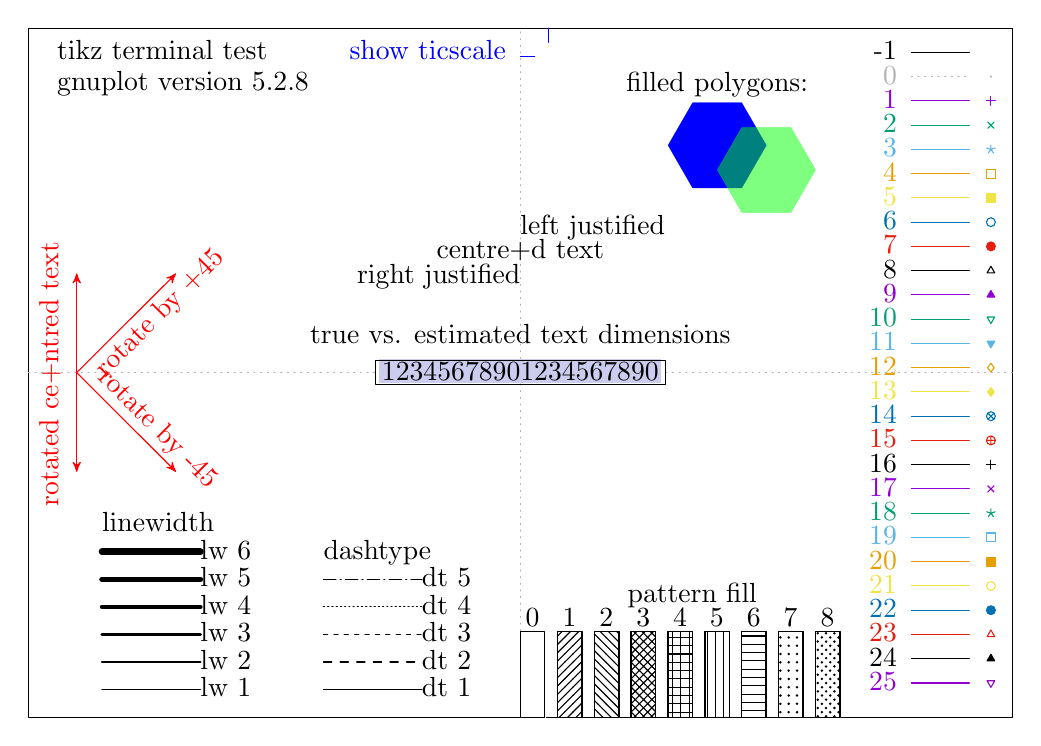
\begin{tikzpicture}[gnuplot]
%% generated with GNUPLOT 5.2p8 (Lua 5.3; terminal rev. Nov 2018, script rev. 108)
%% 2021年05月10日 22時42分14秒
\path (0.000,0.000) rectangle (12.500,8.750);
\gpcolor{color=gp lt color border}
\gpsetlinetype{gp lt border}
\gpsetdashtype{gp dt solid}
\gpsetlinewidth{1.00}
\draw[gp path] (0.000,0.000)--(12.499,0.000)--(12.499,8.749)--(0.000,8.749)--cycle;
\node[gp node left,inner sep=0pt](gp boxed node 62) at (0.368,8.442) {tikz  terminal test};
\node[gp node left,inner sep=0pt](gp boxed node 63) at (0.368,8.057) {gnuplot version 5.2.8  };
\gpcolor{color=gp lt color axes}
\gpsetlinetype{gp lt axes}
\gpsetdashtype{gp dt axes}
\draw[gp path] (6.250,0.000)--(6.250,8.749);
\draw[gp path] (0.000,4.375)--(12.499,4.375);
\gpcolor{color=gp lt color border}
\node[gp node center,inner sep=0pt](gp boxed node 1) at (6.250,4.375) {12345678901234567890};
\gpcolor{rgb color={0.800,0.800,0.933}}
\gpsetlinetype{gp lt border}
\gpsetdashtype{gp dt solid}
\node[fill={}, inner xsep=1.00, inner ysep=1.00,fit=(gp boxed node 1)]{};
\gpcolor{color=gp lt color border}
\node[gp node center,inner sep=0pt](gp boxed node 2) at (6.250,4.375) {12345678901234567890};
\node[gp node center,inner sep=0pt](gp boxed node 3) at (6.250,4.837) {true vs. estimated text dimensions};
\draw[gp path] (4.410,4.529)--(8.090,4.529)--(8.090,4.221)--(4.410,4.221)--cycle;
\node[gp node left,inner sep=0pt](gp boxed node 4) at (6.250,6.223) {left justified};
\node[gp node center,inner sep=0pt](gp boxed node 5) at (6.250,5.915) {centre+d text};
\node[gp node right,inner sep=0pt](gp boxed node 6) at (6.250,5.607) {right justified};
\gpcolor{color=gp lt color 2}
\gpsetlinetype{gp lt plot 2}
\draw[gp path] (6.610,8.749)--(6.610,8.570);
\draw[gp path] (6.250,8.390)--(6.430,8.390);
\node[gp node right,inner sep=0pt](gp boxed node 7) at (6.066,8.442) {show ticscale};
\gpcolor{color=gp lt color border}
\node[gp node right,inner sep=0pt](gp boxed node 8) at (11.032,8.442) {-1};
\gpsetlinetype{gp lt border}
\draw[gp path] (11.216,8.442)--(11.952,8.442);
\gpcolor{color=gp lt color axes}
\node[gp node right,inner sep=0pt](gp boxed node 9) at (11.032,8.134) {0};
\gpsetlinetype{gp lt axes}
\gpsetdashtype{gp dt axes}
\draw[gp path] (11.216,8.134)--(11.952,8.134);
\gpsetpointsize{4.00}
\gppoint{gp mark 0}{(12.226,8.134)}
\gpcolor{rgb color={0.580,0.000,0.827}}
\node[gp node right,inner sep=0pt](gp boxed node 10) at (11.032,7.826) {1};
\gpsetlinetype{gp lt border}
\gpsetdashtype{gp dt solid}
\draw[gp path] (11.216,7.826)--(11.952,7.826);
\gppoint{gp mark 1}{(12.226,7.826)}
\gpcolor{rgb color={0.000,0.620,0.451}}
\node[gp node right,inner sep=0pt](gp boxed node 11) at (11.032,7.518) {2};
\draw[gp path] (11.216,7.518)--(11.952,7.518);
\gppoint{gp mark 2}{(12.226,7.518)}
\gpcolor{rgb color={0.337,0.706,0.914}}
\node[gp node right,inner sep=0pt](gp boxed node 12) at (11.032,7.210) {3};
\draw[gp path] (11.216,7.210)--(11.952,7.210);
\gppoint{gp mark 3}{(12.226,7.210)}
\gpcolor{rgb color={0.902,0.624,0.000}}
\node[gp node right,inner sep=0pt](gp boxed node 13) at (11.032,6.902) {4};
\draw[gp path] (11.216,6.902)--(11.952,6.902);
\gppoint{gp mark 4}{(12.226,6.902)}
\gpcolor{rgb color={0.941,0.894,0.259}}
\node[gp node right,inner sep=0pt](gp boxed node 14) at (11.032,6.594) {5};
\draw[gp path] (11.216,6.594)--(11.952,6.594);
\gppoint{gp mark 5}{(12.226,6.594)}
\gpcolor{rgb color={0.000,0.447,0.698}}
\node[gp node right,inner sep=0pt](gp boxed node 15) at (11.032,6.286) {6};
\draw[gp path] (11.216,6.286)--(11.952,6.286);
\gppoint{gp mark 6}{(12.226,6.286)}
\gpcolor{rgb color={0.898,0.118,0.063}}
\node[gp node right,inner sep=0pt](gp boxed node 16) at (11.032,5.978) {7};
\draw[gp path] (11.216,5.978)--(11.952,5.978);
\gppoint{gp mark 7}{(12.226,5.978)}
\gpcolor{rgb color={0.000,0.000,0.000}}
\node[gp node right,inner sep=0pt](gp boxed node 17) at (11.032,5.670) {8};
\draw[gp path] (11.216,5.670)--(11.952,5.670);
\gppoint{gp mark 8}{(12.226,5.670)}
\gpcolor{rgb color={0.580,0.000,0.827}}
\node[gp node right,inner sep=0pt](gp boxed node 18) at (11.032,5.362) {9};
\draw[gp path] (11.216,5.362)--(11.952,5.362);
\gppoint{gp mark 9}{(12.226,5.362)}
\gpcolor{rgb color={0.000,0.620,0.451}}
\node[gp node right,inner sep=0pt](gp boxed node 19) at (11.032,5.054) {10};
\draw[gp path] (11.216,5.054)--(11.952,5.054);
\gppoint{gp mark 10}{(12.226,5.054)}
\gpcolor{rgb color={0.337,0.706,0.914}}
\node[gp node right,inner sep=0pt](gp boxed node 20) at (11.032,4.746) {11};
\draw[gp path] (11.216,4.746)--(11.952,4.746);
\gppoint{gp mark 11}{(12.226,4.746)}
\gpcolor{rgb color={0.902,0.624,0.000}}
\node[gp node right,inner sep=0pt](gp boxed node 21) at (11.032,4.438) {12};
\draw[gp path] (11.216,4.438)--(11.952,4.438);
\gppoint{gp mark 12}{(12.226,4.438)}
\gpcolor{rgb color={0.941,0.894,0.259}}
\node[gp node right,inner sep=0pt](gp boxed node 22) at (11.032,4.130) {13};
\draw[gp path] (11.216,4.130)--(11.952,4.130);
\gppoint{gp mark 13}{(12.226,4.130)}
\gpcolor{rgb color={0.000,0.447,0.698}}
\node[gp node right,inner sep=0pt](gp boxed node 23) at (11.032,3.822) {14};
\draw[gp path] (11.216,3.822)--(11.952,3.822);
\gppoint{gp mark 14}{(12.226,3.822)}
\gpcolor{rgb color={0.898,0.118,0.063}}
\node[gp node right,inner sep=0pt](gp boxed node 24) at (11.032,3.514) {15};
\draw[gp path] (11.216,3.514)--(11.952,3.514);
\gppoint{gp mark 15}{(12.226,3.514)}
\gpcolor{rgb color={0.000,0.000,0.000}}
\node[gp node right,inner sep=0pt](gp boxed node 25) at (11.032,3.206) {16};
\draw[gp path] (11.216,3.206)--(11.952,3.206);
\gppoint{gp mark 1}{(12.226,3.206)}
\gpcolor{rgb color={0.580,0.000,0.827}}
\node[gp node right,inner sep=0pt](gp boxed node 26) at (11.032,2.898) {17};
\draw[gp path] (11.216,2.898)--(11.952,2.898);
\gppoint{gp mark 2}{(12.226,2.898)}
\gpcolor{rgb color={0.000,0.620,0.451}}
\node[gp node right,inner sep=0pt](gp boxed node 27) at (11.032,2.590) {18};
\draw[gp path] (11.216,2.590)--(11.952,2.590);
\gppoint{gp mark 3}{(12.226,2.590)}
\gpcolor{rgb color={0.337,0.706,0.914}}
\node[gp node right,inner sep=0pt](gp boxed node 28) at (11.032,2.282) {19};
\draw[gp path] (11.216,2.282)--(11.952,2.282);
\gppoint{gp mark 4}{(12.226,2.282)}
\gpcolor{rgb color={0.902,0.624,0.000}}
\node[gp node right,inner sep=0pt](gp boxed node 29) at (11.032,1.974) {20};
\draw[gp path] (11.216,1.974)--(11.952,1.974);
\gppoint{gp mark 5}{(12.226,1.974)}
\gpcolor{rgb color={0.941,0.894,0.259}}
\node[gp node right,inner sep=0pt](gp boxed node 30) at (11.032,1.666) {21};
\draw[gp path] (11.216,1.666)--(11.952,1.666);
\gppoint{gp mark 6}{(12.226,1.666)}
\gpcolor{rgb color={0.000,0.447,0.698}}
\node[gp node right,inner sep=0pt](gp boxed node 31) at (11.032,1.358) {22};
\draw[gp path] (11.216,1.358)--(11.952,1.358);
\gppoint{gp mark 7}{(12.226,1.358)}
\gpcolor{rgb color={0.898,0.118,0.063}}
\node[gp node right,inner sep=0pt](gp boxed node 32) at (11.032,1.050) {23};
\draw[gp path] (11.216,1.050)--(11.952,1.050);
\gppoint{gp mark 8}{(12.226,1.050)}
\gpcolor{rgb color={0.000,0.000,0.000}}
\node[gp node right,inner sep=0pt](gp boxed node 33) at (11.032,0.742) {24};
\draw[gp path] (11.216,0.742)--(11.952,0.742);
\gppoint{gp mark 9}{(12.226,0.742)}
\gpcolor{rgb color={0.580,0.000,0.827}}
\node[gp node right,inner sep=0pt](gp boxed node 34) at (11.032,0.434) {25};
\draw[gp path] (11.216,0.434)--(11.952,0.434);
\gppoint{gp mark 10}{(12.226,0.434)}
\gpcolor{color=gp lt color 0}
\gpsetlinetype{gp lt plot 0}
\draw[gp path,<->](0.616,3.115)--(0.616,5.635);
\draw[gp path,->](0.616,4.375)--(1.876,5.635);
\draw[gp path,->](0.616,4.375)--(1.876,3.115);
\node[gp node center,rotate=-270,inner sep=0pt](gp boxed node 35) at (0.308,4.375) {rotated ce+ntred text};
\node[gp node left,rotate=45,inner sep=0pt](gp boxed node 36) at (0.924,4.375) {  rotate by +45};
\node[gp node left,rotate=-45,inner sep=0pt](gp boxed node 37) at (0.924,4.375) {  rotate by -45};
\gpcolor{color=gp lt color border}
\gpsetlinetype{gp lt border}
\draw[gp path] (0.937,0.350)--(2.187,0.350);
\node[gp node left,inner sep=0pt](gp boxed node 38) at (2.187,0.350) {  lw 1};
\gpsetlinewidth{2.00}
\draw[gp path] (0.937,0.700)--(2.187,0.700);
\node[gp node left,inner sep=0pt](gp boxed node 39) at (2.187,0.700) {  lw 2};
\gpsetlinewidth{3.00}
\draw[gp path] (0.937,1.050)--(2.187,1.050);
\node[gp node left,inner sep=0pt](gp boxed node 40) at (2.187,1.050) {  lw 3};
\gpsetlinewidth{4.00}
\draw[gp path] (0.937,1.400)--(2.187,1.400);
\node[gp node left,inner sep=0pt](gp boxed node 41) at (2.187,1.400) {  lw 4};
\gpsetlinewidth{5.00}
\draw[gp path] (0.937,1.750)--(2.187,1.750);
\node[gp node left,inner sep=0pt](gp boxed node 42) at (2.187,1.750) {  lw 5};
\gpsetlinewidth{6.00}
\draw[gp path] (0.937,2.100)--(2.187,2.100);
\node[gp node left,inner sep=0pt](gp boxed node 43) at (2.187,2.100) {  lw 6};
\node[gp node left,inner sep=0pt](gp boxed node 44) at (0.937,2.450) {linewidth};
\gpsetdashtype{gp dt 1}
\gpsetlinewidth{1.00}
\draw[gp path] (3.750,0.350)--(5.000,0.350);
\node[gp node left,inner sep=0pt](gp boxed node 45) at (5.000,0.350) {  dt 1};
\gpsetdashtype{gp dt 2}
\draw[gp path] (3.750,0.700)--(5.000,0.700);
\node[gp node left,inner sep=0pt](gp boxed node 46) at (5.000,0.700) {  dt 2};
\gpsetdashtype{gp dt 3}
\draw[gp path] (3.750,1.050)--(5.000,1.050);
\node[gp node left,inner sep=0pt](gp boxed node 47) at (5.000,1.050) {  dt 3};
\gpsetdashtype{gp dt 4}
\draw[gp path] (3.750,1.400)--(5.000,1.400);
\node[gp node left,inner sep=0pt](gp boxed node 48) at (5.000,1.400) {  dt 4};
\gpsetdashtype{gp dt 5}
\draw[gp path] (3.750,1.750)--(5.000,1.750);
\node[gp node left,inner sep=0pt](gp boxed node 49) at (5.000,1.750) {  dt 5};
\node[gp node left,inner sep=0pt](gp boxed node 50) at (3.750,2.100) {dashtype};
\node[gp node center,inner sep=0pt](gp boxed node 51) at (8.434,1.555) {pattern fill};
\def\gpfillpath{(6.250,0.000)--(6.562,0.000)--(6.562,1.093)--(6.250,1.093)--cycle}
\gpfill{color=gpbgfillcolor} \gpfillpath;
\gpfill{color=gp lt color border,gp pattern 0,pattern color=.} \gpfillpath;
\gpsetdashtype{gp dt solid}
\draw[gp path] (6.250,0.000)--(6.250,1.093)--(6.562,1.093)--(6.562,0.000)--cycle;
\node[gp node center,inner sep=0pt](gp boxed node 52) at (6.406,1.247) { 0};
\def\gpfillpath{(6.718,0.000)--(7.030,0.000)--(7.030,1.093)--(6.718,1.093)--cycle}
\gpfill{color=gpbgfillcolor} \gpfillpath;
\gpfill{color=gp lt color border,gp pattern 1,pattern color=.} \gpfillpath;
\draw[gp path] (6.718,0.000)--(6.718,1.093)--(7.030,1.093)--(7.030,0.000)--cycle;
\node[gp node center,inner sep=0pt](gp boxed node 53) at (6.874,1.247) { 1};
\def\gpfillpath{(7.186,0.000)--(7.498,0.000)--(7.498,1.093)--(7.186,1.093)--cycle}
\gpfill{color=gpbgfillcolor} \gpfillpath;
\gpfill{color=gp lt color border,gp pattern 2,pattern color=.} \gpfillpath;
\draw[gp path] (7.186,0.000)--(7.186,1.093)--(7.498,1.093)--(7.498,0.000)--cycle;
\node[gp node center,inner sep=0pt](gp boxed node 54) at (7.342,1.247) { 2};
\def\gpfillpath{(7.654,0.000)--(7.966,0.000)--(7.966,1.093)--(7.654,1.093)--cycle}
\gpfill{color=gpbgfillcolor} \gpfillpath;
\gpfill{color=gp lt color border,gp pattern 3,pattern color=.} \gpfillpath;
\draw[gp path] (7.654,0.000)--(7.654,1.093)--(7.966,1.093)--(7.966,0.000)--cycle;
\node[gp node center,inner sep=0pt](gp boxed node 55) at (7.810,1.247) { 3};
\def\gpfillpath{(8.122,0.000)--(8.434,0.000)--(8.434,1.093)--(8.122,1.093)--cycle}
\gpfill{color=gpbgfillcolor} \gpfillpath;
\gpfill{color=gp lt color border,gp pattern 4,pattern color=.} \gpfillpath;
\draw[gp path] (8.122,0.000)--(8.122,1.093)--(8.434,1.093)--(8.434,0.000)--cycle;
\node[gp node center,inner sep=0pt](gp boxed node 56) at (8.278,1.247) { 4};
\def\gpfillpath{(8.590,0.000)--(8.902,0.000)--(8.902,1.093)--(8.590,1.093)--cycle}
\gpfill{color=gpbgfillcolor} \gpfillpath;
\gpfill{color=gp lt color border,gp pattern 5,pattern color=.} \gpfillpath;
\draw[gp path] (8.590,0.000)--(8.590,1.093)--(8.902,1.093)--(8.902,0.000)--cycle;
\node[gp node center,inner sep=0pt](gp boxed node 57) at (8.746,1.247) { 5};
\def\gpfillpath{(9.058,0.000)--(9.370,0.000)--(9.370,1.093)--(9.058,1.093)--cycle}
\gpfill{color=gpbgfillcolor} \gpfillpath;
\gpfill{color=gp lt color border,gp pattern 6,pattern color=.} \gpfillpath;
\draw[gp path] (9.058,0.000)--(9.058,1.093)--(9.370,1.093)--(9.370,0.000)--cycle;
\node[gp node center,inner sep=0pt](gp boxed node 58) at (9.214,1.247) { 6};
\def\gpfillpath{(9.526,0.000)--(9.838,0.000)--(9.838,1.093)--(9.526,1.093)--cycle}
\gpfill{color=gpbgfillcolor} \gpfillpath;
\gpfill{color=gp lt color border,gp pattern 7,pattern color=.} \gpfillpath;
\draw[gp path] (9.526,0.000)--(9.526,1.093)--(9.838,1.093)--(9.838,0.000)--cycle;
\node[gp node center,inner sep=0pt](gp boxed node 59) at (9.682,1.247) { 7};
\def\gpfillpath{(9.994,0.000)--(10.306,0.000)--(10.306,1.093)--(9.994,1.093)--cycle}
\gpfill{color=gpbgfillcolor} \gpfillpath;
\gpfill{color=gp lt color border,gp pattern 8,pattern color=.} \gpfillpath;
\draw[gp path] (9.994,0.000)--(9.994,1.093)--(10.306,1.093)--(10.306,0.000)--cycle;
\node[gp node center,inner sep=0pt](gp boxed node 60) at (10.150,1.247) { 8};
\gpfill{color=gp lt color 2} (9.375,7.262)--(9.062,7.803)--(8.437,7.803)--(8.125,7.262)%
    --(8.437,6.720)--(9.062,6.720)--cycle;
\gpfill{color=gp lt color 1,opacity=0.50} (10.000,6.950)--(9.687,7.491)--(9.062,7.491)--(8.750,6.950)%
    --(9.062,6.408)--(9.687,6.408)--cycle;
\node[gp node center,inner sep=0pt](gp boxed node 61) at (8.750,8.041) {filled polygons:};
%% coordinates of the plot area
\gpdefrectangularnode{gp plot 1}{\pgfpoint{1.805cm}{1.723cm}}{\pgfpoint{18.655cm}{18.573cm}}
\end{tikzpicture}
%% gnuplot variables

  \end{center}
\end{figure}

\bibliography{ref.bib}
\end{document}